\documentclass[english, Lau, oneside]{sapthesis}%remove "english" for a thesis written in Italian
%Bachelor's (laurea triennale) thesis : Lau 
%Master's (laurea specialistica) thesis: LaM 
%PhD's thesis: PhD 
%\usepackage[italian]{babel} %use this package for a thesis written in Italian
\usepackage[utf8]{inputenx}
\usepackage{indentfirst}
\usepackage{microtype}
%\usepackage{chemformula}
%\usepackage{setspace}
%\usepackage{yfonts,color}
%\usepackage{siunitx}
%\usepackage{comment}
%\usepackage{multirow}
%\usepackage{varioref}
%\usepackage[bottom]{footmisc}
%\usepackage{wrapfig}
%\usepackage{float}
%\usepackage{type1cm}
\usepackage{lettrine}
\linespread{0.9}
%\usepackage{chngcntr}
\usepackage[nottoc, notlof, notlot]{tocbibind}
%\onehalfspacing
%\counterwithout{footnote}{chapter}
\usepackage{hyperref}
\hypersetup{
			hyperfootnotes=true,			
			bookmarks=true,			
			colorlinks=true,
			linkcolor=red,
                        linktoc=page,
			anchorcolor=black,
			citecolor=red,
			urlcolor=blue,
			pdftitle={Empirical survey on graph classification methods for Brain Networks
},
			pdfauthor={Ilaria Taddei},
			pdfkeywords={thesis, sapienza, roma, university}
 }

\title{Empirical survey on graph classification methods for Brain Networks}
\author{Ilaria Taddei}
\IDnumber{1853733}
\course[]{Data Science}
\courseorganizer{Faculty of Information Engineering, Computer Science and Statistics}
\submitdate{2020/2021}
\copyyear{2021}
\advisor{Prof. advisor}
\coadvisor{Dr. co-advisor}
\authoremail{ilariataddei.95@gmail.com}
\examdate{22 September 2015}
\examiner{Prof. ...} \examiner{Prof. ...} \examiner{Prof. ...}  \examiner{Prof. ...}  \examiner{Prof. ...} \examiner{Prof. ...}  \examiner{Prof. ...} 

%we refer to http://ctan.mirrorcatalogs.com/macros/latex/contrib/sapthesis/sapthesis-doc.pdf for an exhaustive description of the sapthesis documentclass.


\begin{document}

\frontmatter
\maketitle

\begin{abstract}
Our brain, as our entire body, is a perfect as complicated machine. For this reason is important to analyse it in an effective and efficient way. An important role in this purpose is given to machine learning and similar algorithmic methods. In fact, many papers have been written on different methods to study the brain as graph or as matrix. Most of all, in those papers they want to recognize if a person is affected by a mental decease, such as, for example, Autism or Schizophrenia.  \\
In this work, the aim is to study and compare some of those methods. First of all is important to have in mind which are the basic elements with which the papers work, such as graphs, classification and brain connectomes. Then, the algorithms taken in consideration can be classified according to the technique used, like Neural Networks or features embeddings. For each method many experiments are made, to see how they work, in which case are more useful, and how good are the results. The experiments are made with different datasets, to see how the methods adapt and how general they are. \\
Future works can be implemented, studying more methods and maybe finding a method that could be easily used by neuroscientists. 
\end{abstract}

\tableofcontents

\mainmatter

\chapter{Introduction}
\label{chap:1}

Neuroscientists, to diagnose a psychiatric disorder, use symptom scores from clinical interviews. For a definitive validation, could be useful to study the interactions between brain regions, in order to see the different behaviours of these interactions in a brain of Typical Developed people and people with disorders. This could be seen through Magnetic Resonance Imaging (MRI), in particular functional MRI (fMRI). The neuroimaging data produced are then pre-processed and transformed in structures that an algorithm can study, in our cases graphs, matrices and time series. From the study of these interactions the important thing that we need to implement is the classification of the brain representation, meaning that each method taken in consideration in this work has the aim to implement a classification that says whether the brain that I give to it is affected by a disorder. This is called brain classification. 

The studies taken in consideration, other than in techniques, differs also in the data that have in input. The inputs could be graphs, matrices, time series and even images. This work is focused on methods that take in input graphs, even in matrix representation. Many methods have been implemented for graph classification. They are important tools that can be applied in many fields and subjects. In our particular field, graph classification of brain networks, becomes important to take in account the structure of the graph, because there could be many brain regions that characterize a specific psychiatric disorder. We will see how in some methods are also studied those regions to identify the once that have different interactions in people with disorders, even if the described experiments of this works are concentrated on the simple classification of brain networks. 

This thesis contains an explanation of the basics with which the study works, then a description of several methods on this subject and then experiments with some of these methods that more represent our field. 

This work was performed during a research internship at ISI Foundation
under the supervision of Dr. Francesco Bonchi.

\section{Outline}
The thesis is organized as follows:

\begin{itemize}
	\item In the current chapter there is an explanation of some basics related to this work.
	\item Chapter \ref{chap:2} contains the classification of the several methods taken in account, so, an overview of the macro-classes of all the implemented techniques to do \emph{graph} and \emph{brain classification}. 
	Then, for each method, there is an explanation of the main characteristics.
	\item Chapter \ref{chap:3} contains the experimental part. Are described the set-up of the experiments, like the datasets and the kind of classification, the results of the experiments and a discussion of the results.
	\item Chapter \ref{chap:4} contains comments about the use of each method and possible future works. 
\end{itemize}

\section{Background}
To understand better all the methods, we should do some explanation of what we will encounter during the lecture. The main arguments we should consider are \textbf{Graphs}, \textbf{Classification} and \textbf{Connectomes}.

\paragraph{Graphs} \
\\
There are many subjects in which graphs are used, and consequently many definitions. In mathematics, a graph is a structured set of objects that, in pairs, could have a relation between themselves. Each object is called a \textit{vertex}, and each relation between a pair of vertices is called an \textit{edge}. So, a graph $ G(V,E) $ is a pair where $ V $ are the vertices and $ E $ are the edges. Graphs are represented in diagram form, where vertices are in circle form and edges are lines that join pairs of vertices with a relation.
\begin{figure}[htbp]
	\centering
	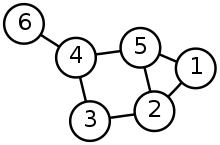
\includegraphics[scale=0.5]{Immagini/220px-6n-graf.svg.png}
	\caption{\label{fig:diagram}}
\end{figure}

Graph could be \textit{directed} or \textit{undirected}. In a direct graph, edges have an orientation, the links between vertices can be represented by arrows going from one vertex to the other. In an edge $ (x,y) $ directed from $ x $ to $ y $, the vertices are called respectively \textit{tail} and \textit{head} of the edge.
\begin{figure}[htbp]
	\centering
	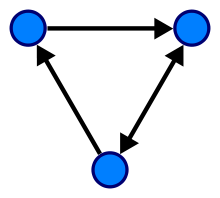
\includegraphics[scale=0.5]{Immagini/220px-Directed.svg.png}
	\caption{\label{fig:diagram2}}
\end{figure}

Graphs can be represented by matrices, the matrix representations in which we are interested for this thesis are \textbf{Adjacency matrix} and/or \textbf{Connectivity matrix}. 

An \textbf{Adjacency matrix} is a square matrix that represents if there is an edge between two vertices. In particular in an unweighted graph with a vertex set $ U=\{u_{1}, ..., u_{n}\} $ the Adjacency matrix $ A $ is an $ n \x n $ matrix in which its element $ A_{ij} $ is 1 if there is an edge between the vertices $ u_{i} $ and $ u_{j} $. If the graph is weighted the values in the matrix are not 1s and 0s, but depends on the weight of each edge. Also, if the graph is undirected the Adjacency matrix is symmetric.

The Adjacency matrix sometimes is called \textbf{Connectivity matrix}.

\paragraph{Classification}\
\\
In machine learning, \emph{Classification} is a supervised learning approach in which an algorithm is trained, with some given data, to classify new observations. It is a process. 

First we have some data, of which we already know the belonging class, called \emph{labelled} data. We could have two classes, in which case we will have a \emph{binary classification}, or multiple classes, so \emph{multi-class classification}. Our labelled data are given to the classification model, starting the \textbf{training} of the model.

Once trained the classificator, we can give to it new data that we want to classify. This is called the \textbf{prediction}. Finished the prediction we can evaluate our model through some scores, the main one in our case is the \textbf{accuracy}, that calculates the percentage of how many predictions of our classifier are right. 

\paragraph{Connectomes}\
\\
The \textbf{connectome} is the connection matrix of the human brain (\cite{connectome}). From the anatomic point of view, the connectome is defined by all the axonal origins, terminations and trajectories of all the brain neurons, through the brain regions. This means, the connectivity of neural pathways in the brain. 

Being able to have a representation of the human brain allows us to understand fundamental cognitive operations, brain activities, conditional structure-function models of the brain, so, consequently, to understand and detect brain deceases. From this powerful tool, we can see how brain physiology is correlated to abilities and behaviours, underlying mental anomalies and pathology. This is fundamental to develop treatments ad hoc for each pathology and case. 

Other fields, that we do not cover here, but that are very interesting, concern the memories (in fact neuroscientists believe that our memories are stored in the synapses between neurons) and the preservation of the brain (being able to recover the structure and connections of it).
https://www.brainpreservation.org/content-2/connectome/

In the following image we can see an example of a connectome.

\begin{figure}[htbp]
	\centering
	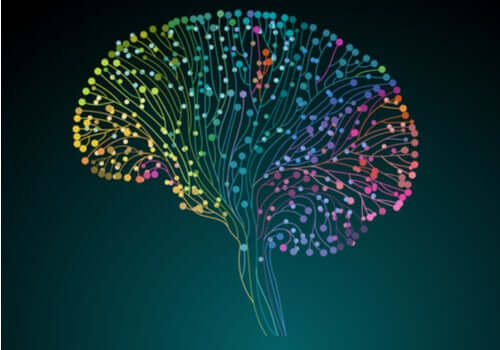
\includegraphics[scale=0.3]{Immagini/cervello-connessioni-neuroni-colorate.jpg}
	\caption{\label{fig:diagram3}}
\end{figure}



\section{Related works}\
\\
Here we concentrate the study of connectomes in graph form. This means that the fMRI of a brain, elaborated in a connectome, is then transformed in graph form, and the graph is studied in matrix form. The graph have as nodes the brain regions, and as edges the connections between them. It follows that the matrix is an \emph{Adjacency matrix}, in which the values represent the degree of connections between the regions, and each row and each column is a node of the graph, a so called \emph{Region of interest} (\textbf{ROI}).
\begin{figure}[htbp]
	\centering
	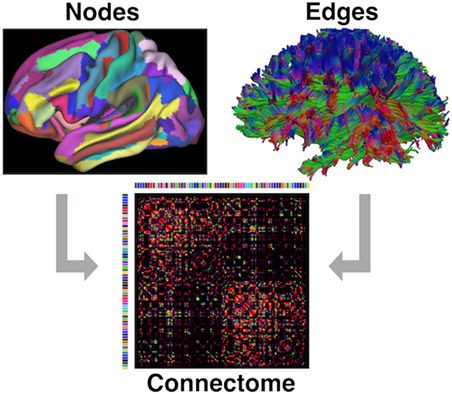
\includegraphics[scale=1]{Immagini/nbm3752-toc-0001-m.jpg}
	\caption{\label{fig:diagram4}}
\end{figure}

\paragraph{Graph Classification}\
\\
The technique that studies the classification of graphs is called \textbf{Graph Classification}. The basic definition of graph classification is (\cite{GraphClassAtt}): given a set of graphs $\mathcal{B}=\left\{\left(\mathcal{G}_{1}, \ell_{1}\right),\left(\mathcal{G}_{2}, \ell_{2}\right), \cdots,\left(\mathcal{G}_{n}, \ell_{n}\right)\right\}$ the aim is to learn a function $f: \mathbf{G} \rightarrow \mathcal{L}$, where $\mathbf{G}$ is the input space of graphs, and $\mathcal{L}$ is the set of graph labels. Each graph $\mathcal{G}_{i}=\left(\mathbf{A}_{\mathcal{G}_{i}}, \mathbf{B}_{\mathcal{G}_{i}}\right)$ has an adjacency matrix $\mathbf{A}_{\mathcal{G}_{i}} \in\{0,1\}^{N_{i} \times N_{i}}$ and an attribute matrix $\mathbf{B}_{\mathcal{G}_{i}} \in\ \mathbf{R}^{N_{i} \times N_{i}}$, where ${N}_{i}$ is the number of nodes of the $i$-graph and $B$ is the number of attributes. Each graph has also a corresponding label $l_{i}$. 	

The usual strategy to study graphs is to calculate graph statistics on the entire graph. A popular technique is to count the occurrences of various \textit{subgraphs} on a graph, called graphlet kernel \cite{pmlr-v5-shervashidze09a}. Then there is the \textit{Morgan algorithm} \cite{Rogers2010ECFP} that consists in an iterative process, that updates the attributes vector of each node by hashing a concatenation of all the attributes of in the node's local neighbourhood. Then from the final attributes of all the nodes in the graph is computed the graph feature. Recently, learning data-driven graph features \cite{NIPS2015_f9be311e} is becoming more important. This means that given a dataset, the task-relevant features are learned automatically from the graphs. Once we extract these features, independently of which method we would like to use, we use them for the classification.
Another method that we can mention is all the literature that regards \textit{Graph Neural Networks} (GNN), a deep learning technique. To build a GNN we need to find out the graph structure, the graph type and its scale, then we should define the loss function, depending on the task, and then we are ready to build a model using computational model \cite{ZHOU202057}. 

These methods brings us to the field of our interest, \textbf{Brain Classification}. For Brain Classification have been used the previous graph classification techniques, adapted for a more suitable result. In the next chapter we will discuss various methods that inspired this work.

\chapter{Survey}
\label{chap:2} 

\section{All methods}
In this chapter there will be a brief description of some papers that treated \textit{brain classification}. We can divide the methods in the several techniques that the papers use to build the brain classification: Deep Learning, Statistical Fingerprints and Machine Learning. Also, to compare them, and find a possible good way to make brain classification, some have been tested. The results are in chapter \ref{chap:3}.

\subsection{Deep Learning}
\paragraph{GroupINN: Grouping-based Interpretable Neural Network for Classification of Limited, Noisy Brain Data}\
\\

This paper of Yan Y. et al \cite{groupinn} proposes a grouping-based interpretable neural network model, GroupINN, that classifies cognitive performance with 85\% fewer parameters than baseline deep models, while also identifying the most predictive brain subnetworks within several task-specific contexts. In the design of the neural network is included the idea of node grouping. In this way the model learns the node grouping and extracts the graph features jointly.
\\

The problem statement of this paper is: given a set of subjects, each with corresponding fMRI data and a label associated with a certain phenotype, we seek to devise an efficient, interpretable, and parsimonious neural network model that can predict each phenotype with high accuracy.
\\

To reduce the number of parameters used in the model, they adopted the idea of multi-graph clustering (where the goal is to find a common clustering across multiple graphs) to summarize the original graph into a supergraph with each cluster as a supernode. 
\\

The neural network is formed by three different types of layers: node grouping layer, graph convolutional layer and fully connected layer. The node grouping layer is designed to “hide” the non-indicative (‘noisy’) edges by grouping them into a cluster, thus highlighting the indicative edges: two nodes are assigned to different groups if their connection is identified as important.
Graph convolutional layers are used to capture the structure of the supergraph.
\\

The neural network is also divided in two branches, one processes the positive graphs and one the negative ones. 
All in all, the architecture consists of three kinds of layers and two branches. 
The input graph is the correlation matrix $W$. The first layer is a dimensionality reduction layer and the output is a matrix $W^{s}$ representing the supergraph. Following the dimensionality reduction layer, three graph convolutional layers are used. At last, the positive and negative outputs of the previous layer are concatenated, flattened and sent to the fully connected layer (with softmax activation).

\begin{figure}[htbp]
	\centering
	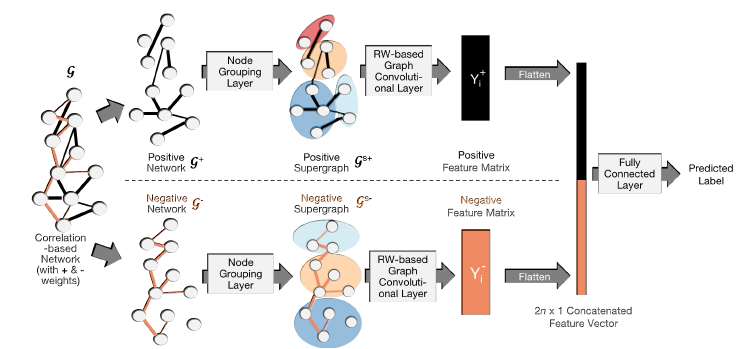
\includegraphics[scale=0.8]{Immagini/Groupinn1.PNG}
	\caption{\label{fig:diagram5}}
\end{figure}

Regarding the experimentation part, they used a dataset taken from Human Connectome Project 1200 (HCPt) \cite{hcp}. 
This dataset consists of 966 subjects to which has been measured brain activity, through fMRI, while they were performing specific tasks. The four task-based datasets used in this experiment are: \textit{Emotion, Gambling, Social} and \textit{Working Memory}. It is divided in 90\% train/validation set and 10\% testing set. For the evaluation they take in consideration \textit{accuracy} and the \textit{runtime}. Comparing their method, they found out that it is faster and with less parameters than other works, so it is more interpretable, as well as having good accuracy.
\\

\paragraph{Deep Learning-based Pipeline to Recognize Alzheimer’s Disease using fMRI Data}\
\\

S. Sarraf et al. \cite{Sarraf066910} built a Neural Network, specifically a Convolutional Neural Network (\textbf{CNN}) for classification of clinical data, in particular they tested it for Alzheimer disease. Their dataset is composed of a group of people affected by Alzheimer and a control group. They where scanned with resting-state FMRI, and after a preprocess, the data consisted of images of functional information. 
\\

CNNs in general are used to study images, and are composed of Pooling layers, Normalization layers, Fully Connected layers and Convolutional layers. Convolutional layers help to maintain the spacial order of the input they are working on, obviously very important on images, and these layers consist on filters applied to these images. In this case they used an already implemented CNN called LeNet-5 (by Y. LeCun et al \cite{726791}), and adjusted it for FMRI data. The data in input were 2D images, that were labeled for binary classification, as shown in figure \ref{fig:diagram7}.

\begin{figure}[htbp]
	\centering
	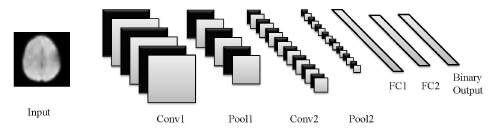
\includegraphics[scale=1]{Immagini/deep-learning1.PNG}
	\caption{\label{fig:diagram7}}
\end{figure}

The experiment ended up with a very high accuracy (96.8588\%) and a very low learning rate, meaning that it is a valid tool, even if on one hand it is a very complicated model, has many parameters and hyperparameters to tune and could have GPU memory problems.

\paragraph{Functional Brain Network Classification for Alzheimer’s Disease Detection with Deep Features and Extreme Learning Machine}\
\\

X. Bi et al \cite{Bi2019FunctionalBN} designed two deep learning methods of functional brain network classification. More precisely they concentrate their work on Alzheimer disease detection. The first model is a Convolutional learning method, that learns the deep regional-connectivity features. The second is a Recurrent learning method, learning deep adjacent positional features. So, both the learning methods are Neural Networks. They also implemented an Extreme Learning Machine (ELM) to improve the learning ability, and is implemented in the learning methods.
\\

Both the deep learning methods take as input a graph matrix, i.e. the adjacency matrix of each patient. 
The Convolutional Learning method \ref{fig:diagram8} is composed of a Convolutional layer, Activation function, Pooling layer, Fully Connected layer and a Decision layer. It is in the Convolutional layer that the features are extracted, while in the decision layer, with a \textit{Softmax} function, are generated the labels of each brain network.

\begin{figure}[htbp]
	\centering
	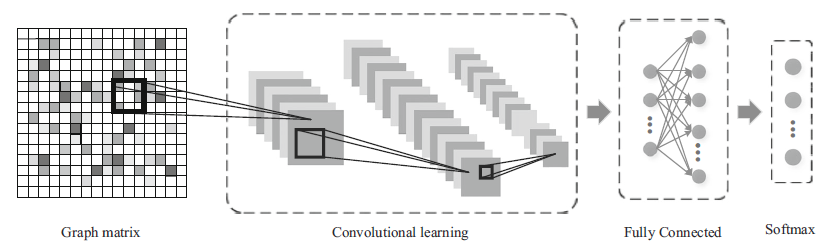
\includegraphics[scale=0.5]{Immagini/functional1.PNG}
	\caption{\label{fig:diagram8}}
\end{figure}

To the Recurrent learning method \ref{fig:diagram9} is given as input a row o more of the graph matrix at each time step, until all the rows are learned. It is mainly composed of two parts, the recurrent structure and the classification structure. 

\begin{figure}[htbp]
	\centering
	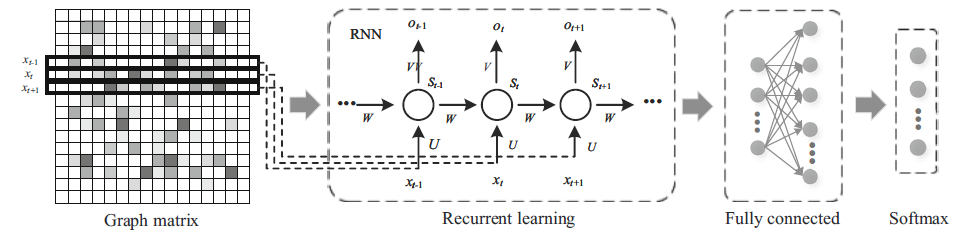
\includegraphics[scale=0.5]{Immagini/functional2.PNG}
	\caption{\label{fig:diagram9}}
\end{figure}

The complexity of these two models is in the fully connected layer, where there is an high computation for the parameters tuning. For this reason is built the ELM layer. It is much faster and gives good generalization performance. So, the deep features are extracted, convolutional or recurrent ones, and are given to the ELM layer, that produces the output labels \ref{fig:diagram10}. 

\begin{figure}[htbp]
	\centering
	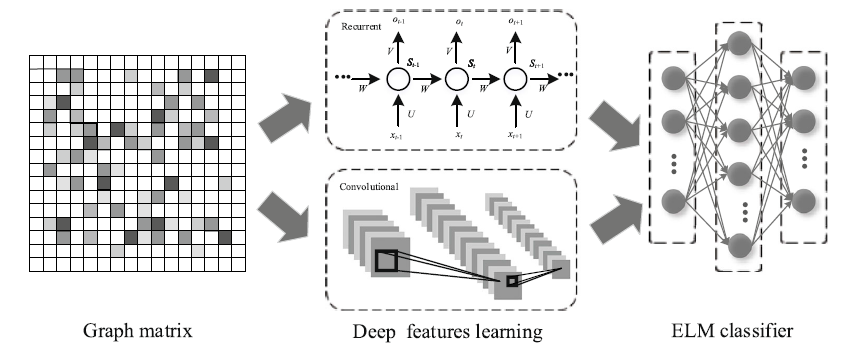
\includegraphics[scale=0.5]{Immagini/functional3.PNG}
	\caption{\label{fig:diagram10}}
\end{figure}

For the experiments they compared their methods with shallow methods. They saw that, with ELM, both neural networks performed better than without ELM, but ELM also brings performance fluctuation. Anyway, they performed much better than shallow methods. Recurrent method, in particular, is slightly better that the Convolutional one, but takes much more training time. Instead, Convolutional learning method, having more parameters to tune, reaches with more difficulty the optimal performance.

\subsection{Statistical Fingerprints}
\paragraph{Explainable Classification of Brain Networks via Contrast Subgraphs}\
\\

In this work of Bonchi F, Lanciano T. and Gionis A. \cite{lanciano2020cs} they introduce an approach for classifying brain networks based on extracting contrast subgraphs, i.e., a set of vertices whose induced subgraphs are dense in one class of graphs and sparse in the other. The model is extremely simple, with just one parameter, excellent interpretability and good classification accuracy. What they want to improve or add, differently from others methods, are the node-identity awareness, black box effect and high number of parameters. With \textbf{node-identity awareness} is meant to take in consideration that a specific vertex corresponds to the same ROI in all the input graphs. This is very important to find similarities among the input networks. The majority of the models have a \textbf{black box effect}, meaning that are complicated to understand how to use them, and their parameters. It should be crucial to make it understandable for neuroscientists that need these tools. Even the \textbf{high number of parameters} could be a problem, for overfitting and for tuning them. 
\\

Let's go more in details. Each individual is represented by an undirected unweighted graph with $|V|$ = 116 vertices, that are the ROIs. This means that for each patient we have a squared correlation matrix of 116 rows and columns. They exploits two problems regarding contrast-subgraphs, in the experiments chapter \ref{chap:3} we will mention only the first one. \textit{Problem 1} states that given the observations of condition group - affected by autism - and control group, and the corresponding summary graphs, they seek to find a subset of vertices that maximizes the contrast-subgraph objective, so to find a set of vertices whose induced subgraph is dense in the summary graph of $G^{\mathcal{A}}$ - condition group - and sparse in summary graph $G^{\mathcal{B}}$ - control group. It can be summarised in the following equation:
\begin{equation}
	\delta(S)=e^{\mathcal{A}}(S)-e^{\mathcal{B}}(S)-\alpha\left(\begin{array}{c}
		|S| \\
		2
	\end{array}\right)
\end{equation}
where $ e^{\mathcal{A}}(S) $ and $ e^{\mathcal{B}}(S) $ correspond to the number of edges in the subgraph induced by $ S $ in the summary graphs $G^{\mathcal{A}}$ and $G^{\mathcal{B}}$, and $ \alpha $ is a parameter that penalize large size solutions: larger the value of $\alpha$, smaller is the optimal contrast-subgraph. 
\\

\textit{Problem 2} is a symmetric variant, wanting to find a subgraph having the largest absolute difference of edge weights between $G^{\mathcal{A}}$ and $G^{\mathcal{B}}$, so that maximize the contrast-subgraph. 
\\

Calculating constrast-subgraph TD-ASD and ASD-TD from a dataset they used to make experiments, they were able to observe differences between the two graphs.
\begin{figure}[htbp]
	\centering
	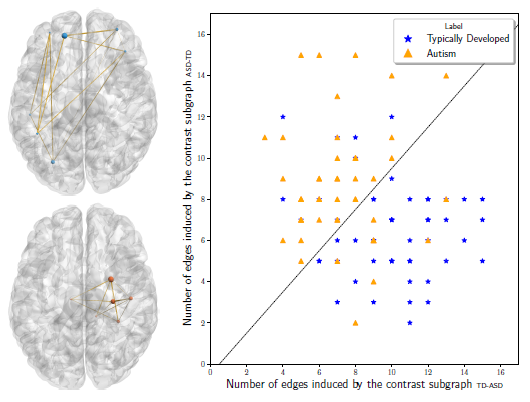
\includegraphics[scale=0.8]{Immagini/c-s1.PNG}
	\caption{\label{fig:diagram6}}
\end{figure}
They ended up with figure \ref{fig:diagram6}, where the top left image is the TD-ASD contrast-subgraph, while the bottom left image is the ASD-TD contrast-subgraph. We can clearly see the patterns differences between the two contrast-subgraphs. Also, from the right part of the image \ref{fig:diagram6}, we have a scatterplot with number of edges induces by TD-ASD - x axis - and ASD-TD - y axis - for each patient. With these results they ended up with some important rules:
\begin{itemize}
	\item If an individual exhibits more than 62 edges among the 15 vertices of the contrast subgraph ASD-TD, then there are high chances that the individual is affected by ASD;
	\item If the number of edges induced by the contrast subgraph ASD-TD is smaller than half of the number of edges induced by the contrast subgraph TD-ASD, then there are high chances that the individual is not affected by ASD;
	\item If the number of edges induced by the contrast subgraph ASD-TD is smaller than the number of edges induced by the contrast subgraph TD-ASD, then there are high chances that the individual is affected by ASD.
\end{itemize}

They used these two features to make classification, based on SVM, and compared the results with other methods of the literature. At the end they have a single parameter $\alpha$, a very low run-time (less than 30 seconds to extract the constrast-subgraph), a simple explainability, having only two simple features, and high accuracy. 

\paragraph{Unsupervised Network Embedding for Graph Visualization, Clustering and Classification}\
\\

A crucial challenge in mining network-based data is to find effective ways to represent or encode graph structures, in order to make themm efficiently exploited by Machine Learning algorithms. L. Gutiérrez et al \cite{GutierrezUn} provide an unsupervised approach to learn embedding representation for a collection of graphs, to use in graph mining tasks. They use an unsupervised neural network on graphs that aims to capture the distribution of the data, to discriminate between different class of networks. With their method, they learn automatically a feature representation of graphs assessing their similarity on an Euclidean space \ref{fig:diagram11}, focusing on problems defined on networks that account for \textit{node identity}. They evaluate the method in three network mining tasks: graph clustering, graph classification and visualization. We are more interested in graph classification.

\begin{figure}[htbp]
	\centering
	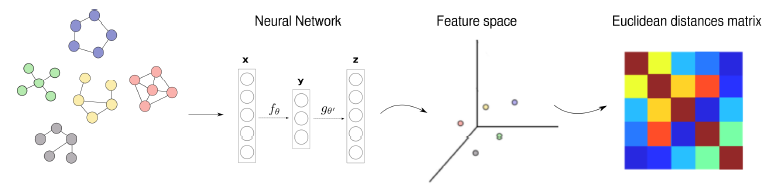
\includegraphics[scale=0.5]{Immagini/Unsupervised.PNG}
	\caption{\label{fig:diagram11}}
\end{figure}


Unlike classical distances in the literature, such as \textit{Hamming} and \textit{Jaccard} distances, this approach performs network comparisons directly on a feature space, through a learned non-linear mapping applied to input graphs. It is composed by some blocks. The first is the \textbf{Autoencoder}, that is one of the most popular unsupervised neural network approaches. Unsupervised approaches aim to uncover hidden patterns or learning representations from unlabeled data. In particular, the autoencoder allows to compress the representation of input data, removing redundancy and reducing the dimension of the input. A traditional autoencoder learns a non-linear mapping which encodes an input example in a smaller dimensional latent vector. Unfortunately, this method could just learn the training data, meaning that it will not work on unknown data. For this reason they train a \textbf{Denoising Autoencoder} (\textbf{DAE}) \ref{fig:diagram12}, that reconstruct a clean or repaired version from corrupted input.

\begin{figure}[htbp]
	\centering
	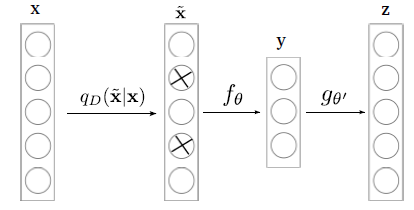
\includegraphics[scale=0.5]{Immagini/unsupervised2.PNG}
	\caption{\label{fig:diagram12}}
\end{figure}
 
Giving in input an adjacency matrix to the DEA could be insufficient, so they compute higher powers of the matrix to capture multiple path relationships. Also, this method remains invariant to the node ordering when the same node permutation is assigned to the graph, having a collection of networks with node correspondence across graphs. A main advantage of transforming graphs into feature vectors is that it allows to compare easily networks computing only Euclidean distances between their
embeddings.
\\

For the experiment part, we will see the graph classification results. Their task is to classify connectomes according to gender, male or female. The input is a dataset built from MRI, structural and diffusion, so a collection of graphs. The two steps of the model are learning graph embedding through DAE and computation of a pairwise Euclidean distance matrix. Comparing their method with classic ones of the literature, they saw that it outperformed them, at accuracy level, remaining competitive only with DeltaCon model. Regarding the runtime, it is much faster than all the others.
\paragraph{Supervised classification of structural brain networks reveals gender differences}\
\\

Another work base on statistical fingerprint is the one of Chiem B. et al \cite{8379106}. The work aims to study individual differences in the structural connectome, not the functional one, with perfect node correspondence property. This property means that each node corresponds to the same anatomical location in each connectome. They propose three new methods based on SVM.
\\

The first contribution of this paper regards the feature extraction, crucial point for the classification part. They introduced the \textbf{Bag-of-Edges}, it consists in the application of the \textit{Recursive Feature Eliminatio} (RFE). It trains an SVM with linear kernel, sorts features according to the weights granted by the SVM, and reduces the size of the feature vector keeping only a percentage of the most discriminative features. It stops when a given number of features is reached \ref{fig:diagram13}. At the end we have a feature vector with only the most discriminative edges of the graph.

\begin{figure}[htbp]
	\centering
	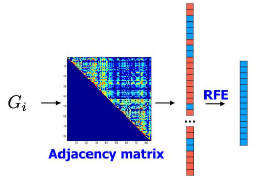
\includegraphics[scale=0.8]{Immagini/supervised1.PNG}
	\caption{\label{fig:diagram13}}
\end{figure}
 
To take advantage of perfect node property they designed two new graph kernels. First they used the \textbf{DeltaCon Kernel}, introduced by Koutra et al \cite{koutra2013deltacon}, but never used as a kernel. As first step they compute for each graph a node-to-node affinity matrix, that encodes a particular measure of similarity between nodes of the graph. The similarity measure taken in consideration is Fast Belief Propagation (FaBP). Then is defined the DeltaCon kernel similarity between two graphs \ref{fig:diagram14}. 

\begin{figure}[htbp]
	\centering
	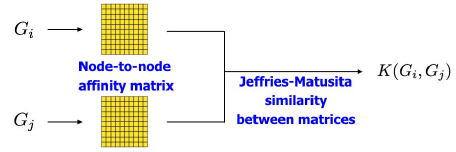
\includegraphics[scale=0.8]{Immagini/supervised2.PNG}
	\caption{\label{fig:diagram14}}
\end{figure}

The second graph kernel is the kernel based on \textbf{regularized Laplacian}. It follows the same principle of the DeltaCon kernel, but uses a different similarity measure, the regularized Laplacian.
\\

The experiments aim to classify connectomes, detecting the gender of the brain in input. The method that gave better results is the Bag-of-edges, even if even the other two models performed better than other graph kernels take from the literature. In particular, the DeltaCon kernel worked better with regularized Laplacian similarity.

\paragraph{Sub-network Kernels for Measuring Similarity of Brain Connectivity Networks in Disease Diagnosis}\
\\

The innovation of this paper of B. Jie \cite{Jie2018} is in the fact that they take in consideration both global and local properties of brain regions to construct graph kernels for measuring the similarity of brain networks. They propose a novel sub-network kernel on brain networks for brain decease classification. They first construct a group of sub-networks on each node to reflect the multi-level connectivity properties of brain networks. Then, we define the similarity of a pair of brain networks, by calculating the similarities of all corresponding pairs of sub-network groups when considering the uniqueness of nodes. The total contribution of this work comprehend three steps: a novel sub-network kernel for measuring the similarity between brain networks, a sub-network kernel based learning (SKL) framework for automated brain disease diagnosis based on fMRI data and finally an implementation for performing inference on brain network data.
\\

The proposed \textbf{sub-network kernel based learning} (\textbf{SKL}) framework for brain disease classification in composed by the following steps: 

\begin{enumerate}
	\item Image preprocessing and connectivity network construction;
	\item Network thresholding and sub-network kernel construction;
	\item Classification.
\end{enumerate}

It is illustrated in figure \ref{fig:diagram15}.

\begin{figure}[htbp]
	\centering
	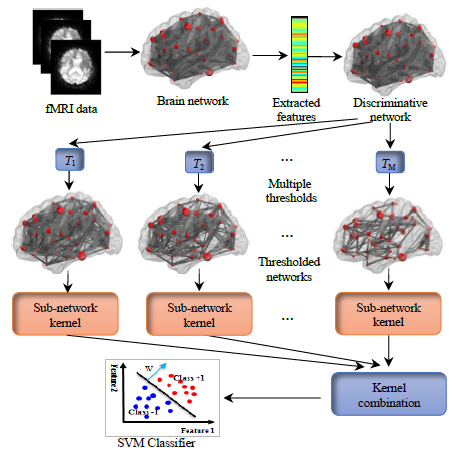
\includegraphics[scale=0.8]{Immagini/subnetwork1.PNG}
	\caption{\label{fig:diagram15}}
\end{figure}

After the preprocess of the images, there is the construction of sub-network kernel. First a group of sub-networks is constructed on each node to reflect the multi-level connectivity properties of the brain. Then is calculated the similarity between brain networks. It is done calculating the similarity of all pairs of sub-networks groups from the same node across different brain networks, since each node on each brain network corresponds to the same ROI. 
\\

The sub-network kernel based Learning starts with a \textit{discrimination} of the nodes to construct more discriminative networks. It is done with \textit{t}-test and a thresholding with \textit{p}-value. The result is a feature vector that represents the discriminative network. Then there is a \textit{network thresholding}, with different thresholds, that will remove edges with zero weights, to reflect the topological properties of discriminative networks. Eventually, having more thresholds, they adopt a \textit{multi-kernel SVM classification} with grid-search approach. Once found the optimal parameters, the traditional SVM can be applied for classification.
\\

Compared with others state-of-the-art kernels, this method performs much better, with higher accuracy and AUC. They also experimented on different parameters. The two parameters to tune are \textit{d}, the number of iterations to compute the mathematical representation of sub-networks, and \textit{h}, the size of a sub-network set. They saw that \textit{h} is very important, because they reached the best performance at $ h = 2 $, while for \textit{d} the method is robust. 
Another important evidence is that, without constructing discriminative networks from the originals brain network, the model is not so accurate compared to the model with it. 

\paragraph{Integration Of Network Topological Features And Graph Fourier Transform For Fmri Data Analysis}\
\\

Very interesting is the new approach of J. Wang et al \cite{8363530}. Their challenge is to evaluate differences of functional connectivity networks between different age groups. The novelty is in the fact that the brain networks are constructed combining commonly used topological features from complex network analysis, with \textbf{Graph Fourier Transform} (GFT). GFT contributes to find the significant subspace of the original signal, so it could be a complementary information, given the fact that topological features reveal the morphological structure of the brain network. 

\begin{figure}[htbp]
	\centering
	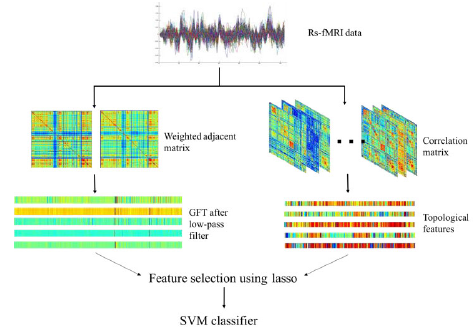
\includegraphics[scale=0.8]{Immagini/integration.PNG}
	\caption{\label{fig:diagram16}}
\end{figure}

In \textit{Graph signal}, resting-state fMRI data can be viewed as time series graoh signals defined on the parcellated brain regions. On each graph can be computed the GFT, and the eigenvalues are taken in consideration for the construction of the network. To represent the original graph signal, are selected the low frequency components, corresponding to the first several eigenvalues calculated by GFT. 
\\

For the topological features they calculate the \textit{centrality} and the \textit{segregation}. The centrality of the nodes is calculated with two measures, the degree and the betweeness centrality. The segregation refers to the existence of specialized neurons and brain areas, organized into distinct neural populations and grouped together to form segregated cortical areas. Functional segregation in the brain is the ability for specialized processing to occur within these areas. A simple measure of functional segregation is defined based on the number of triangles in the network, with a high number of triangles implying segregation.
\\

To construct the graph, once calculated the topological features, they concatenate the data into a $ 264 x (TM) $ matrix, where M is the number of subjects. Each row is normalized into a unit norm. To estimate the adjacency matrix is used the Gaussian radial basis functional kernel. Then they can get the features from the frequency domain by GFT. 
\\

After the construction of the input data, they use a regularized least-square regression using lasso algorithm for feature selection. The features are then given to a linear SVM classifier. The results of the experiment gives high accuracy, but they where not compared with other state-of-the-art methods. The steps of the model are illustrate in figure \ref{fig:diagram16}.

\subsection{Machine Learning}
\paragraph{Network Classification With Applications To Brain Connectomics}\
\\


\paragraph{Stable Biomarker Identification For Predicting Schizophrenia in the Human Connectome}\
\\

Stable Biomarker Identification model \cite{GutierrezBio} is one of the methods we will take in account for the experimentation part. They adopt a machine learning approach that aims at discovering the most relevant set of biomarkers for discriminating subjects groups and thus quantitatively describing the group differences, both in terms of classification accuracy and stability of selected features. 
\\

Biomarkers discovery consists on the identification of regions or connections of interest associated with a neural disorder. From machine learning perspective, the choice of biomarkers can be addressed as a feature selection problem. They perform an automatic feature selection procedure in order to identify biomarkers that are relevant for the diagnosis of schizophrenia from brain connectivity data. As a classifier they use an RFE-SVM, integrated into an embedded feature selection approach. The aim of the present work is threefold:

\begin{itemize}
	\item First, they investigate the effect of structural, functional, and multi-modal (structural+functional) connectome with different resolutions in the classification performance of schizophrenia.
	\item Second, they perform a careful feature selection procedure across modalities in order to assess the robustness of the selected features providing the best trade-off between high accuracy and stability. 
	\item Finally, the analysis of retrieved biomarkers allows to identify a distributed set of brain regions engaged in the discrimination of patients and control subjects.
\end{itemize}  

As we can see in figure \ref{fig:diagram18} the model has two Cross Validation. The outer CV, represented by the left image, is used to evaluate the performance of the model. The inner CV, at the right part of the image, is used to choose the best parameters for the classification.

\begin{figure}[htbp]
	\centering
	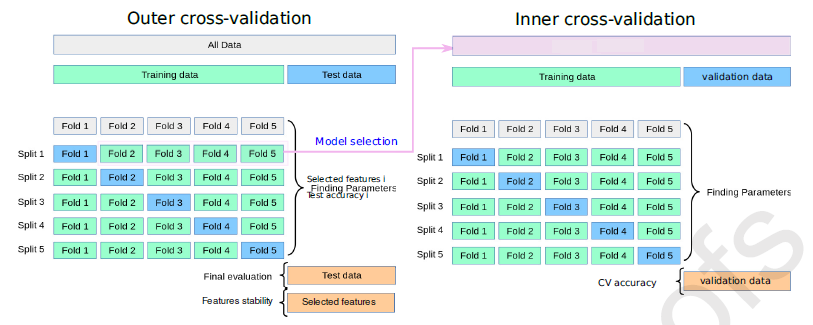
\includegraphics[scale=0.65]{Immagini/stablebiomarkers.PNG}
	\caption{\label{fig:diagram18}}
\end{figure}



\paragraph{Multi-modality disease modelling via collective deep matrix factorization}\
\\

This model of Q. Wang et al \cite{10.1145/3097983.3098164} is based on a framework to fuse multiple data modalities for predictive modeling, using deep matrix factorization. In particular, they study three modalities together, two kinds of MRI and genetic data. The first type of MRI is \textbf{T1 MRI}, that capture structural information of grey matter in the brain. The other is the diffusion-weighted MRI (\textbf{dMRI}), that is sensitive to microscopic properties of brain's white matter. So, T1 MRI captures areas composed of neurons while dMRI estimated connections between those area. The genotype impacts the disease in a way that is not directly related to brain structure and function. All these modalities interact in a complicated manner, this suggests that directly combining feature spaces may not lead to effective integration.
\\

To reduce the feature dimensionality while maintaining most information they use \textbf{matrix factorization technique}. Traditional matrix factorizations assume linear interactions between data. This cannot be the case, there are non-linear interactions. They propose a deep matrix factorization framework to fuse information from multiple modalities and transfer predictive knowledge to differentiate patients with mild cognitive impairment (MCI), early stage of Alzheimer, from cognitive normal subjects. They build a non-linear hierarchical deep matrix factorization framework which decomposes each modality into a modality invariant component and a modality specific component, guided by supervision information. 
\\

To fuse multiple data modalities through deep matrix factorization they use a deep neural network to factorize each modality. The structure is illustrated in figure \ref{fig:diagram17}.

\begin{figure}[htbp]
	\centering
	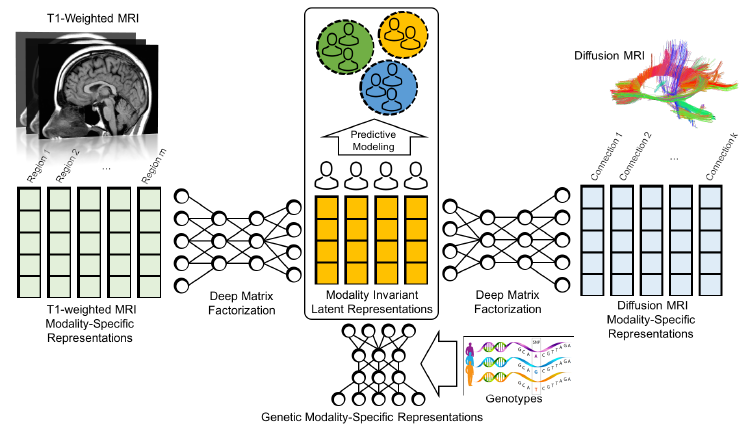
\includegraphics[scale=0.65]{Immagini/multimodality.PNG}
	\caption{\label{fig:diagram17}}
\end{figure}

The deep neural network serves as highly non linear mapping between the input matrix and the factorized matrix, and projects the latent representations non-linearly to the same latent space. 
They saw that with the fusion of all the three modalities the performance are higher than when they use only one or two modalities, and also outperforms other matrix factorization methods.



\chapter{Experiments}
\label{chap:2}
\section{Experimental setup}
With datasets explanation

\section{Results}
(Data Science)

\section{Discussion}
\label{sec:moons}
 

\chapter{Conclusions}

\section{Future works}

\backmatter
\phantomsection
\begin{thebibliography}{17}

\bibitem{ref:vph}
Blanche P.A., Gailly P., et al., “\textit{Volume phase holographic gratings: large size and high diffraction efficiency}“, Optical Engineering, Vol. 43, No.11, November 2004

\bibitem{ref:science}
Cirasuolo M., et al., \textit{"MOONS Science Report"}, MOONS Document Number: VLT-TRE-MON-14620-0001, Issue: $1.0$, $31^{\textup{st}}$ January $2013$

\bibitem{ref:eso}
European Southern Observatory, \url{http://www.eso.org}

\end{thebibliography}

\end{document}